\documentclass[border=10pt]{standalone}
\usepackage{tikz}\usepackage{amsmath}\usetikzlibrary{arrows.meta}
\begin{document}
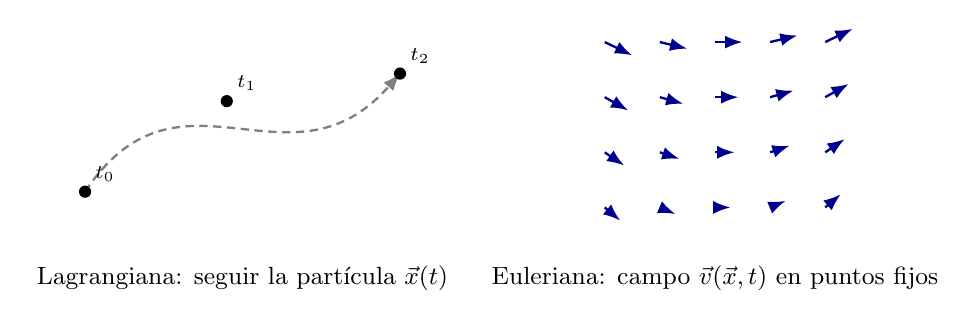
\begin{tikzpicture}[line width=0.85pt,>={Latex[length=2.2mm]}]
  % Lagrangiana: seguir la particula
  \draw[gray,densely dashed,->] (-2,-0.8) .. controls (-0.8,1.0) and (0.6,-0.9) .. (2,0.7);
  \foreach \t/\x/\y in {0/-2/-0.8, 1/-0.2/0.35, 2/2/0.7}{
    \fill (\x,\y) circle(2.2pt); \node[above right] at (\x,\y){\scriptsize $t_\t$};}
  \node at (0,-1.9){\small Lagrangiana: seguir la partícula $\vec x(t)$};
  % Euleriana: campo en puntos fijos
  \begin{scope}[xshift=6cm]
    \foreach \x in {-1.4,-0.7,0,0.7,1.4} \foreach \y in {-1,-0.3,0.4,1.1}{
       \pgfmathsetmacro{\u}{0.45+0.12*\y}\draw[->,blue!55!black] (\x,\y)--++(\u*0.6,0.12*\x);}
    \node at (0,-1.9){\small Euleriana: campo $\vec v(\vec x,t)$ en puntos fijos};
  \end{scope}
\end{tikzpicture}
\end{document}
